\section*{Ejercicio 1}
\graphicspath{{Figuras/}}

En la parte superior de la Figura \ref{01:fig:rasterplot} se observa la envolvente del estímulo al que fue sometido el receptor acústico del saltamontes. En la zona inferior, se observan las respuestas a este estímulo para cada una de las 128 realizaciones. indicando con un punto en aquellas ventanas de tiempo en los cuales se obtuvo un spike. Se observa que para algunas ventanas de tiempo, por ejemplo para $t\approx 400\,\text{ms}$, en donde la densidad de spikes es claramente menor que durante el resto del estímulo.

\begin{figure}[h!]
    \centering
    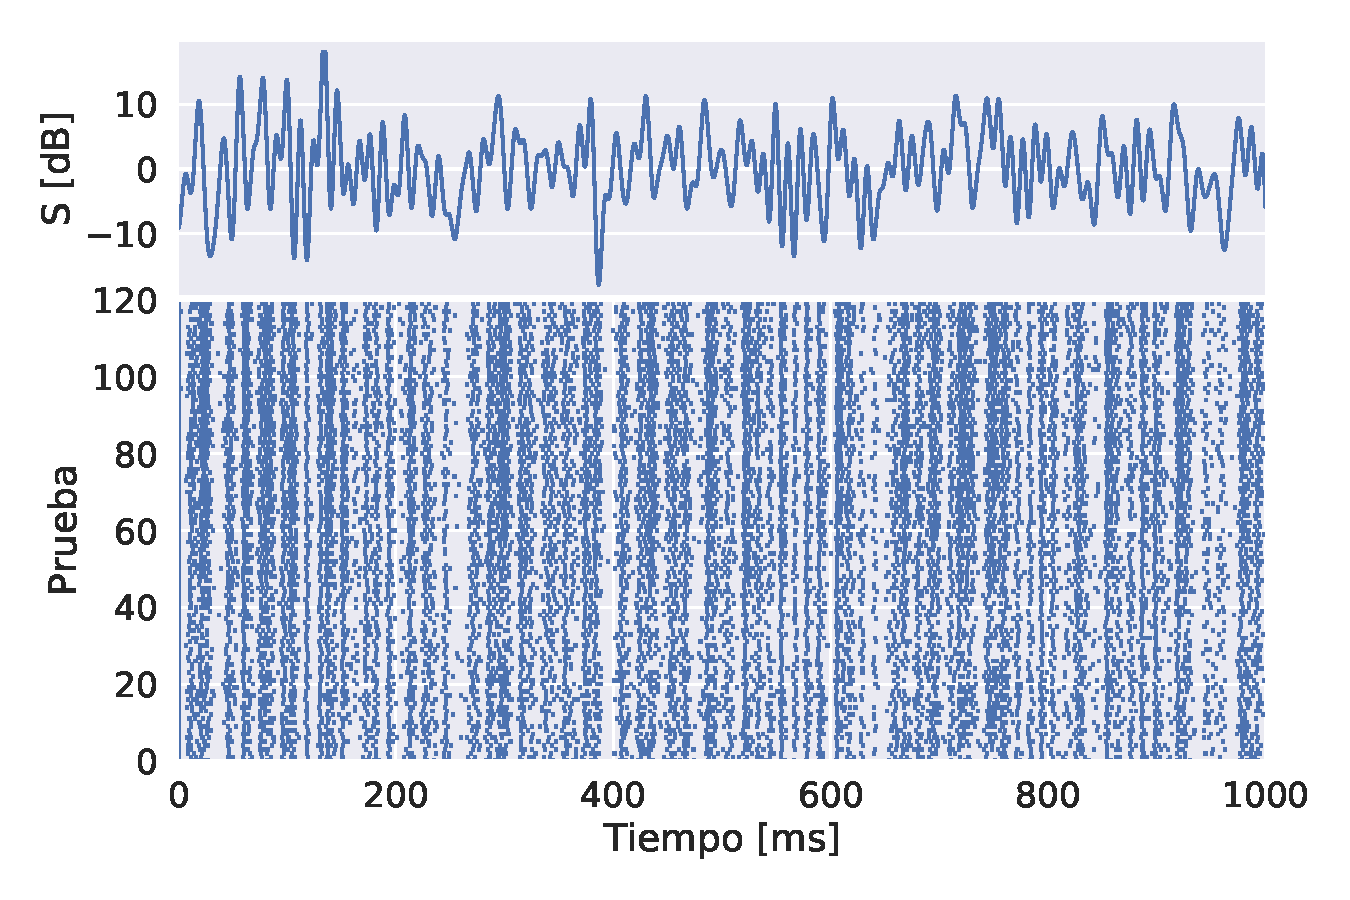
\includegraphics[width=0.9\textwidth]{1_Rasterplot.pdf}
    \caption{En la figura superior, se observa el estímulo utilizado en función del tiempo. En la figura inferior, se observa con un punto los momentos en donde se presento un spike en la actividad del saltamontes, para cada una de las 128 realizaciones.}
    \label{01:fig:rasterplot}
\end{figure}

En la Figura \ref{01:fig:histograma} se observa una histograma que aproxima la distribución ISI (\textit{inter-spike interval}), considerando las 128 realizaciones. En la misma, se observa que luego de un spike, la neurona no vuelve a disparar por uno pocos milisegundos. Esto se debe a que al llegar un potencial de acción, se abren los canales de sodio y se desporaliza la neurona. Luego los canales de sodio se inactivan hasta que la bomba ATPasa vuelve a polarizar la membrana y reactiva los canales de sodio, con lo cual la neurona no puede recibir ningún potencial de acción nuevo durante este periodo de tiempo, generalmente denominado periodo refractario.



\begin{figure}[h!]
    \centering
    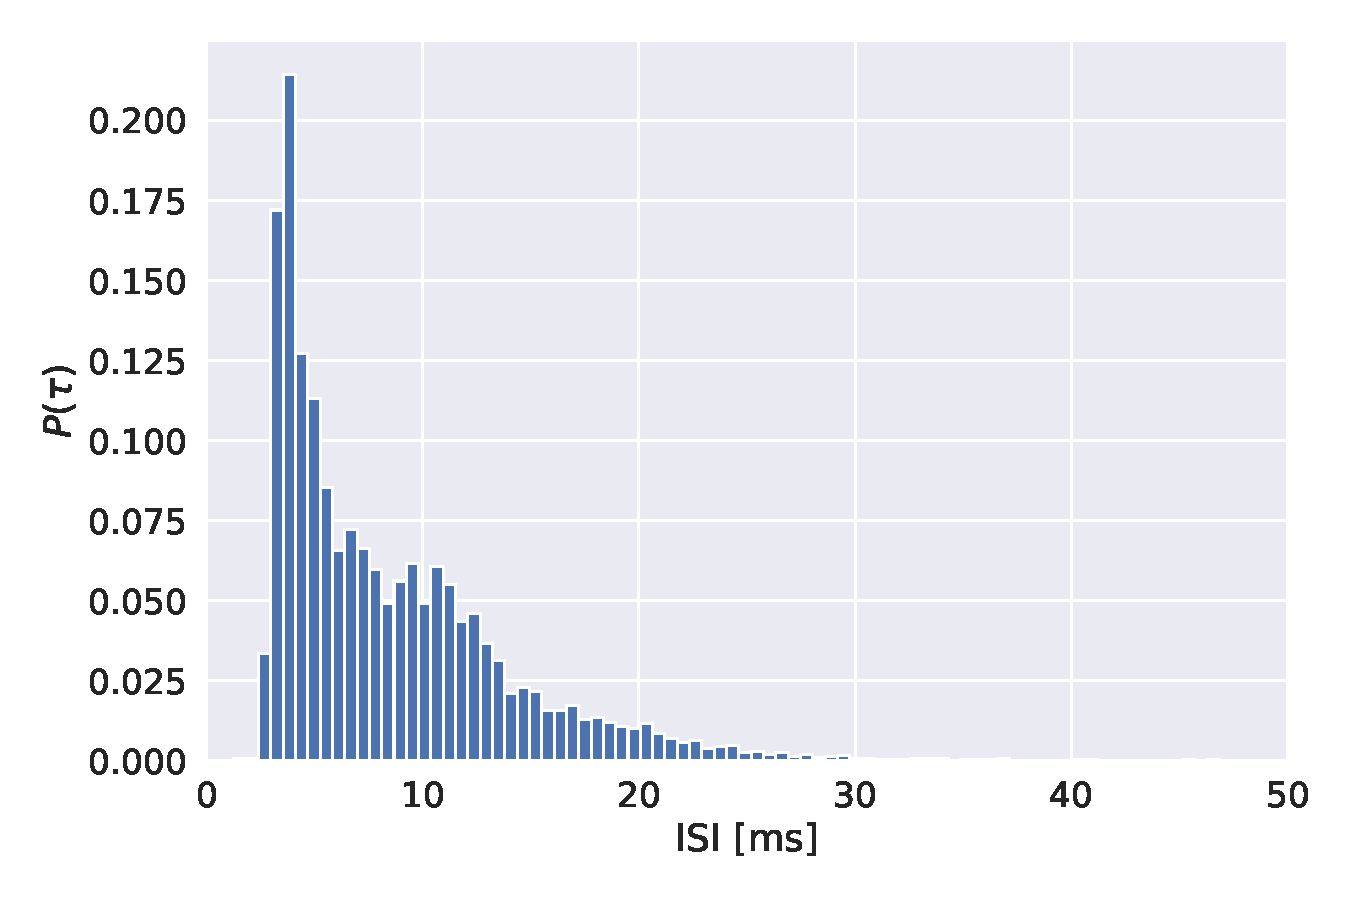
\includegraphics[width=0.8\textwidth]{1_Distr_ISI.pdf}
    \caption{Histograma normalizado que aproxima la distribución $P(\tau)$ en función del ISI (\textit{inter-spike interval}), considerando las 128 realizaciones.}
    \label{01:fig:histograma}
\end{figure}

Luego se calculo el coeficiente de variabilidad ($CV$), para el cual se obtuvo que $CV\approx0.657$. Dado que $CV \neq 1$, podemos concluir que este proceso no es un proceso de Poisson. Esta conclusión también puede desprenderse del hecho que la distribución de ISI obtenida en la Figura \ref{01:fig:histograma} no se corresponde con una distribución exponencial decreciente.